\section{Layout}

Com os resultados de simulação validando o funcionamento do circuito, foi possível iniciar o desenvolvimento do layout. Todo o projeto foi realizado utilizando a ferramenta \textit{Virtuoso}, da \textit{Cadence}, utilizando o processo \textit{TSMC CMOS 180 nm}. O circuito integrado apresentado na \autoref{fig_circintegrado} foi desenvolvido, contendo todo o projeto de Receptor Óptico além de outros projetos desenvolvido por outros alunos\footnote{"Projeto de um Oscilador em Anel Controlado por Tensão de Múltiplas Saídas em Tecnologia CMOS 180 nm" \cite{VictorRodrigues}}\footnote{"Projeto de um Conversor CC-CC CMOS para Aplicações de Energy Harvesting" \cite{LucasChaves}}. A \autoref{fig_circintegrado_division} mostra de maneira explicita o que representa cada parte do CI. O circuito integrado apresenta uma área total de 2x2 mm² (2,56 mm²), utilizando um encapsulamento do tipo CLCC44\footnote{Especificações do encapsulamento presentes no \autoref{anexo_clcc44}}. A \autoref{tab_clcc44} apresenta a relação da numeração dos pinos do encapsulamento com os pinos chip, que são distintos, além da identificação de cada pino. A \autoref{tab_clcc44_2} apresenta outros pinos presente no encapsulamento, referente à outros trabalhos.

\begin{figure}[htb]
 \centering
    \caption{Circuito Integrado utilizado para o Receptor Óptico} 
    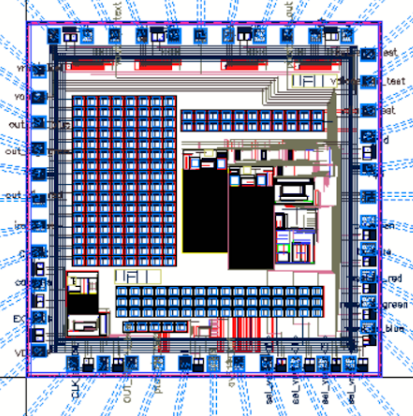
\includegraphics[scale=0.5]{Resultados/Imagens/CircuitoIntegrado.png}
    \legend{Fonte: Produzido pelo autor}
    \label{fig_circintegrado}
\end{figure}

\begin{figure}[htb]
 \centering
    \caption{Circuito Integrado utilizado para o Receptor Óptico particionado} 
    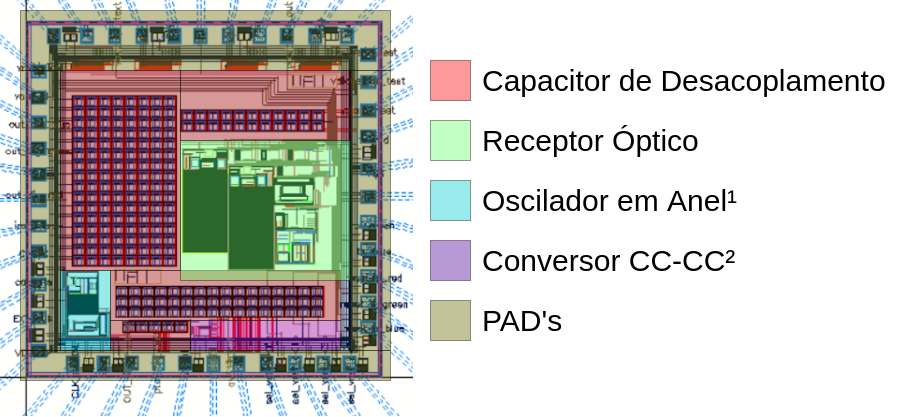
\includegraphics[scale=0.4]{Resultados/Imagens/Image_CircuitoIntegrado.png}
    \legend{Fonte: Top View desenvolvido por Daniel Carvalho Lott}
    \label{fig_circintegrado_division}
    \nota{¹ Projeto desenvolvido por Victor Rodrigues Barbosa \cite{VictorRodrigues}\\² Projeto desenvolvido por Lucas Martins Chaves \cite{LucasChaves}}
\end{figure}

A \autoref{layoutcompleto} apresenta a implementação completa do Receptor Óptico projetado. A \autoref{layoutcompleto_division} mostra a mesma figura explicitando o que representa as diferentes parte do circuito. O projeto do Receptor Óptico ocupa uma área total de 422 633,9x666,96 $\mu$m² (~0,423 mm²).

\begin{figure}[htb]
 \centering
    \caption{Layout completo do circuito desenvolvido} 
    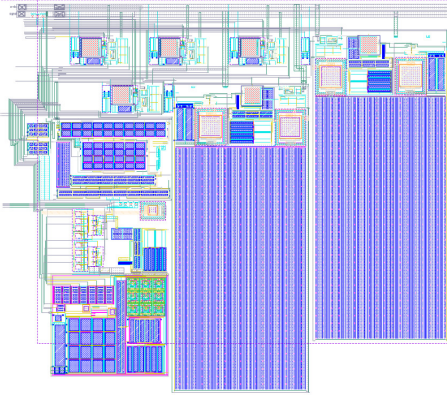
\includegraphics[scale=1, angle = 90]{Resultados/Imagens/Circuito Completo.png}
    \legend{Fonte: Produzido pelo autor}
    \label{layoutcompleto}
    \nota{Imagem rotacionada em 90° em sentido anti-horário}
\end{figure}

\begin{figure}[htb]
 \centering
    \caption{Layout completo do circuito particionado} 
    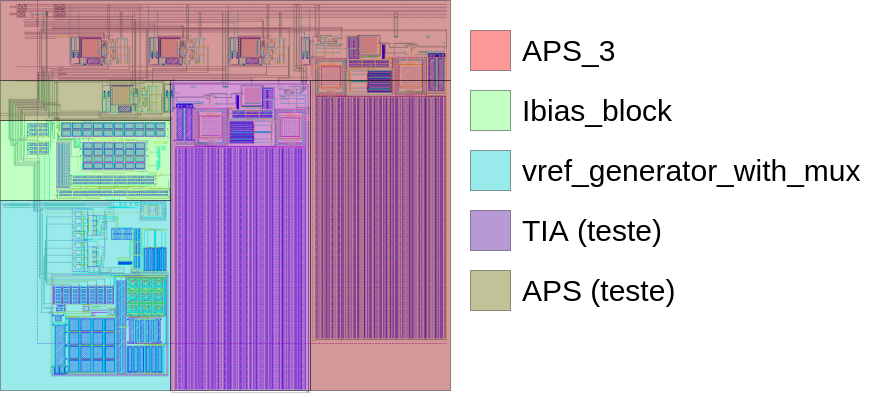
\includegraphics[scale=0.4]{Resultados/Imagens/Image_CircuitoCompleto.png}
    \legend{Fonte: Produzido pelo autor}
    \label{layoutcompleto_division}
\end{figure}

\begin{table}[]
\caption{Pinos presentes no circuito integrado para o Projeto do trabalho apresentado}
\footnotesize
\begin{tabular}{cccll}
\toprule
\begin{tabular}[c]{@{}c@{}}Pino\\ Circuito \\ Integrado\end{tabular} & \begin{tabular}[c]{@{}c@{}}Pino\\ Chip\end{tabular} & Nome              & \multicolumn{1}{c}{Descrição}                                                                           & \multicolumn{1}{c}{Observação} \\
\multicolumn{5}{c}{Projeto Receptor Óptico}                                                                                                                                                                                                                                            \\
\midrule \midrule
1                                                                 & 40                                                  & vref\_pixel       & \begin{tabular}[c]{@{}l@{}}Tensão de referência do APS\\ de teste\end{tabular}                                                                    &                                \\\midrule
2                                                                 & 41                                                  & vout\_clk         & Tensão de saída de relógio gerada                                                                       &                                \\\midrule
3                                                                 & 42                                                  & out\_dig\_blue    & \begin{tabular}[c]{@{}l@{}}Sinal de tensão digital\\ para cor azul\end{tabular}                         &                                \\\midrule
4                                                                 & 43                                                  & out\_dig\_green   & \begin{tabular}[c]{@{}l@{}}Sinal de tensão digital\\ para cor verde\end{tabular}                        &                                \\\midrule
5                                                                 & 44                                                  & VSS               & Terra                                                                                                   &                                \\\midrule
6                                                                 & 1                                                   & out\_dig\_red     & \begin{tabular}[c]{@{}l@{}}Sinal de tensão digital\\ para cor vermelha\end{tabular}                     &                                \\\midrule
7                                                                 & 2                                                   & iref\_test        & ???????????????????                                                                        &                                \\\midrule
23                                                                & 18                                                  & reset\_b\_blue    & \begin{tabular}[c]{@{}l@{}}Sinal de tensão de RESET\\ no APS para cor azul\end{tabular}                 & Ativo em nível baixo           \\\midrule
24                                                                & 19                                                  & reset\_b\_green   & \begin{tabular}[c]{@{}l@{}}Sinal de tensão de RESET\\ no APS para cor verde\end{tabular}                & Ativo em nível baixo           \\\midrule
25                                                                & 20                                                  & reset\_b\_red     & \begin{tabular}[c]{@{}l@{}}Sinal de tensão de RESET\\ no APS para cor vermelha\end{tabular}             & Ativo em nível baixo           \\\midrule
26                                                                & 21                                                  & tx\_blue          & \begin{tabular}[c]{@{}l@{}}Sinal de tensão de ENABLE\\ no APS para cor azul\end{tabular}                & Ativo em nível alto            \\\midrule
27                                                                & 22                                                  & tx\_green         & \begin{tabular}[c]{@{}l@{}}Sinal de tensão de ENABLE\\ no APS para cor verde\end{tabular}               & Ativo em nível alto            \\\midrule
28                                                                & 23                                                  & V18               & Tensão de alimentação de 1,8V                                                                           &                                \\\midrule
29                                                                & 24                                                  & VSS               & Terra                                                                                                   &                                \\\midrule
30                                                                & 25                                                  & tx\_red           & \begin{tabular}[c]{@{}l@{}}Sinal de tensão de ENABLE\\ no APS para cor vermelha\end{tabular}            & Ativo em nível alto            \\\midrule
31                                                                & 26                                                  & vdiode\_test      & \begin{tabular}[c]{@{}l@{}}Corrente que simula um potencial\\ no fotodiodo do APS de teste\end{tabular} &                                \\\midrule
32                                                                & 27                                                  & vdiode\_clk\_test & \begin{tabular}[c]{@{}l@{}}Corrente que simula um potencial\\ no fotodiodo no TIA de teste\end{tabular} &                                \\\midrule
33                                                                & 28                                                  & out\_ana\_test    & \begin{tabular}[c]{@{}l@{}}Sinal de tensão analógico para o\\ APS de teste\end{tabular}                 &         \\\bottomrule                      
\end{tabular}
\label{tab_clcc44}
\legend{Fonte: Produzido pelo autor}
\end{table}

O bloco \textit{APS\_digitalized} projetado é apresentado na figura \autoref{layoutAPSDIG}. A \autoref{layoutAPSDIG_division} mostra a mesma figura explicitando o que representa as diferentes parte do circuito. O projeto do bloco ocupa uma área total aproximada de 3307 $\mu$m².

\begin{figure}[htb]
 \centering
    \centering
    \caption{Layout do bloco \textit{APS\_digitalized}} 
    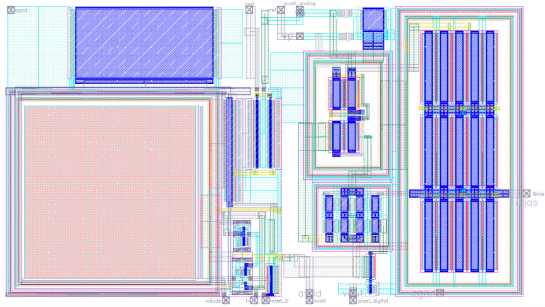
\includegraphics[scale=0.8]{Resultados/Imagens/APS_DIGITALIZED.png}
    \legend{Fonte: Produzido pelo autor}
    \label{layoutAPSDIG}
\end{figure}

\begin{figure}[htb]
 \centering
    \centering
    \caption{Layout do bloco \textit{APS\_digitalized} particionado} 
    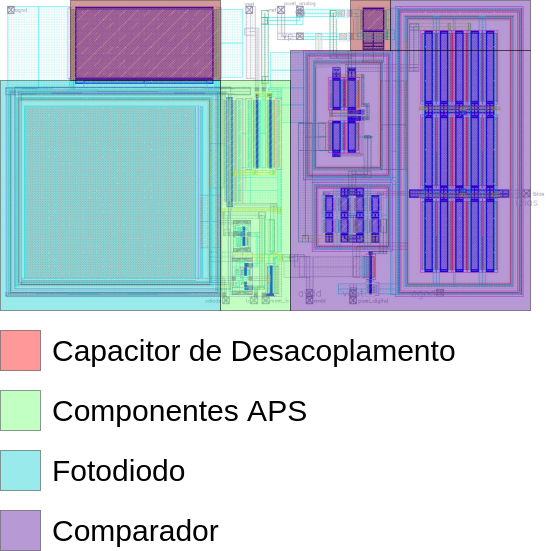
\includegraphics[scale=0.3]{Resultados/Imagens/Image_APS_Digitalized.png}
    \legend{Fonte: Produzido pelo autor}
    \label{layoutAPSDIG_division}
\end{figure}

O bloco \textit{APS\_clk} projetado é apresentado na figura \autoref{layoutTIA}. A \autoref{layoutTIA_division} mostra a mesma figura explicitando o que representa as diferentes parte do circuito. O projeto do bloco ocupa uma área total aproximada de 102107 um².

\begin{figure}[htb]
 \centering
    \begin{minipage}{0.5\textwidth}
    \centering
    \caption{Layout do bloco \textit{APS\_clk}} 
    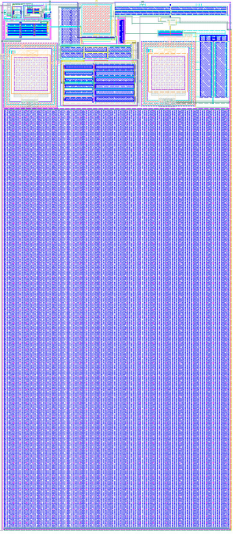
\includegraphics[scale=0.7]{Resultados/Imagens/TIA.png}
    \legend{Fonte: Produzido pelo autor}
    \label{layoutTIA}
    \end{minipage}
    \hfill
    \begin{minipage}{0.4\textwidth}
    \centering
    \caption{Layout do bloco \textit{APS\_clk} particionado}
    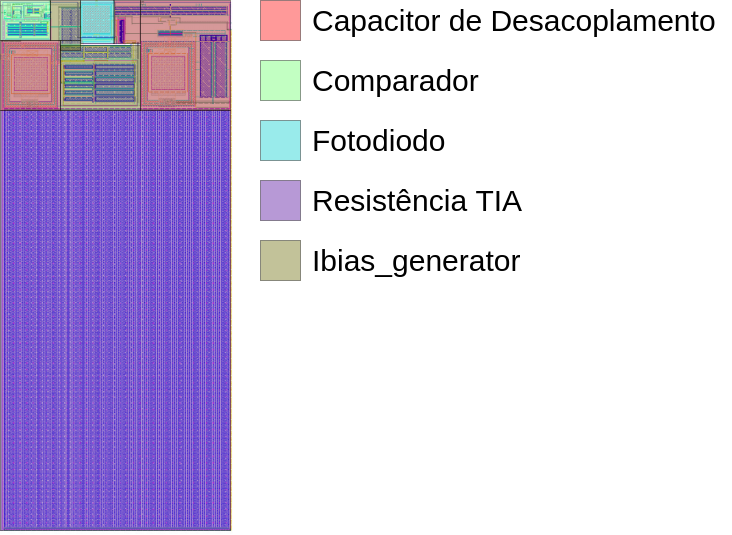
\includegraphics[scale=0.4]{Resultados/Imagens/Image_TIA.png}
    \legend{Fonte: Produzido pelo autor}
    \label{layoutTIA_division}
    \end{minipage}
\end{figure}

O bloco \textit{APS\_3} projetado é apresentado na figura \autoref{layoutAPS_3}. A \autoref{layoutAPS_3_division} mostra a mesma figura explicitando o que representa as diferentes parte do circuito. O projeto do bloco ocupa uma área aproximada de 123353 $\mu$m².

\begin{figure}[htb]
    \centering
    \caption{Layout do bloco \textit{APS\_3}} 
    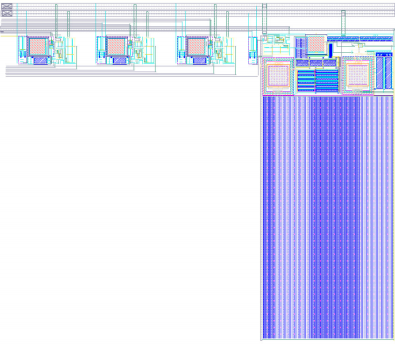
\includegraphics[scale=1]{Resultados/Imagens/APS_3.png}
    \legend{Fonte: Produzido pelo autor}
    \label{layoutAPS_3}
\end{figure}

\begin{figure}[htb]
    \centering
    \caption{Layout do bloco \textit{APS\_3} particionado} 
    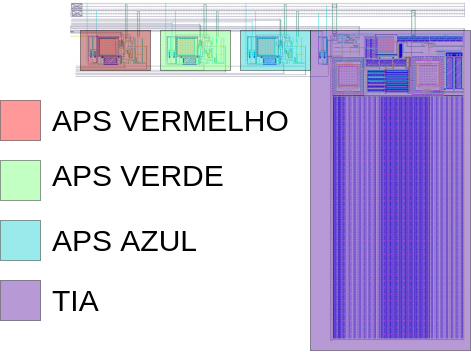
\includegraphics[scale=0.4]{Resultados/Imagens/Image_APS_3.png}
    \legend{Fonte: Produzido pelo autor}
    \label{layoutAPS_3_division}
\end{figure}
